\documentclass[a4paper]{article}
\usepackage[utf8]{inputenc}
\usepackage[T1]{fontenc}
\usepackage[pdftex]{graphicx}
\usepackage{fancyhdr}
\usepackage{lscape}
\usepackage{color}
\usepackage{gensymb}
\usepackage{qtree}
\usepackage[english]{babel}
\usepackage{graphicx}
\usepackage[colorinlistoftodos]{todonotes}
\usepackage{listings}
\usepackage{color}
\usepackage{changepage}
\usepackage[margin=1in]{geometry}
\definecolor{codegreen}{rgb}{0,0.6,0}
\definecolor{codegray}{rgb}{0.5,0.5,0.5}
\definecolor{codepurple}{rgb}{0.58,0,0.82}
\definecolor{backcolour}{rgb}{0.95,0.95,0.92}
\usepackage[final]{pdfpages} 
\usepackage{amssymb}
\usepackage{hyperref}
 
 \lstdefinestyle{mystyle}{
 	backgroundcolor=\color{backcolour},   
 	commentstyle=\color{codegreen},
 	keywordstyle=\color{magenta},
 	numberstyle=\tiny\color{codegray},
 	stringstyle=\color{codepurple},
 	basicstyle=\footnotesize,
 	breakatwhitespace=false,         
 	breaklines=true,                 
 	captionpos=b,                    
 	keepspaces=true,                 
 	numbers=left,                    
 	numbersep=5pt,                  
 	showspaces=false,                
 	showstringspaces=false,
 	showtabs=false,                  
 	tabsize=2
 }
 
\lstset{
	style=mystyle,
	inputencoding=utf8,
	extendedchars=true,
	literate={á}{{\'a}}1 {ã}{{\~a}}1 {é}{{\'e}}1,
	escapechar=\&
}
\title{Notes rapide provenant du livre}
\author{Charles Jacquet 2781-12-00}



\begin{document}
\maketitle

\section{Définition de base}
\begin{itemize}
\item \textbf{Abstraction : }Décomposer un problème jusque dans ses parties les plus fondamentales.

\item \textbf{Abstract Data Type : } C’est un model mathématique de structures de données qui spécifie le type de donnée , les opérations supportées ainsi que les arguments nécessaire pour celles-ci. C'est une sorte de contrat où on dit ce que la structure doit faire mais on ne dit pas comment elle doit le faire.
Pour rendre le ADT plus indépendant de son interface, il est préférable de l'implémenter avec une interface plutot qu'avec une classe.

\item \textbf{Collection : } Une collection d'objet est un ensemble d'objets stoqué avec grâce à une structure particulière.

\item \textbf{Arbre ordonné : } Un arbre est dit ordonné, si il y a une significaiton linéaire à l'ordre des enfants. C'est-à-dire que l'ordre à de l'importance dans le parcourt de l'arbre.

\item \textbf{Arbre binaire impropre : } Un arbre binaire propre est un arbre dont tous les noeuds internes ont soit aucun ou soit deux enfants chacun. Ceci étant dit, un arbre impropre est un arbre qui possède au moins un noeud n'ayant pas exactement deux fils.

\item \textbf{Hauteur d'un arbre : } c'est le nombre maximum de génération en dessous du noeud. Le niveau n, est l'ensemble des noeuds de hauteur n. La feuille (leaf) la plus basse est de hauteur 0.
\item \textbf{Profondeur d'un arbre : } C'est le nombre de parents que possède un noeud. La racine est de profondeur 0.

\item \textbf{Arbre complet : } Un arbre complet est un arbre dont tous les noeuds internes ont exactement deux enfants. Un arbre complet implique que tous les enfants d'un même parent ont la même hauteur. Dès lors, la différence des hauteurs d'enfants ayant le même parent sera toujours égale à 0, donc un arbre complet est toujours équilibré.

\item \textbf{Arbre essentiellement complet : } C'est lorsque tous les noeuds sauf les noeuds du dernier niveau sont complet, c'est à dire qu'ils possèdent le maximum de noeuds. Et ensuite, tous les noeuds du dernier niveau sont au maximum à gauche. Un arbre essentiellement complet est également toujours équilibré.

\item \textbf{Graphe directed : } Chaque edge à un sens.

\item \textbf{Internal node : } Noeud avec au minimum un enfant.

\item \textbf{External node : } Noeud sans enfant.

\item \textbf{Position équilibrée : } Une position dans un arbre est dite balancée si la valeur absolue de la diférence entre la hauteur de ses enfants est au maximum de 1.

\item \textbf{Arbre équilibré : } Un arbre équilibré est un arbre pour lequel la valeur absolue de la différence entre la hauteur du sous-arbre de gauche et de celle du sous-arbre de droite est au maximum de 1.

\item \textbf{Patron de conception : } est un arrangement caractéristique de modules, reconnu comme bonne pratique en réponse à un problème de conception d'un logiciel. Il décrit une solution standard, utilisable dans la conception de différents logiciels.(Wikipédia)

\item \textbf{Weighted Graphs : } Dans certains graphes, un poid est associé à chaque arrêtes.
\end{itemize}

\section{Les itérateurs}
\subsection{snapshot iterator}
L'itérateur maintient sa propre copie la collection
\subsection{lazy iterator}
Ne fait que passer d'un éléments à l'autre avec l'opération next


\section{Array and linked List}

Il exite plusieurs sortes de linked lists:

\subsection{Simple array}
Attention, si on doit trouver des éléments dans un tableau à 2 dimensions avec un algo en O(n log(n)) il suffit de faire un binary search sur les n niveaux. soit N * log(n).

\subsection{Simplement liée}
Contient juste un lien vers l'élement suivant.
Est util pour l'implémentation de stack (pile) ou de queue (queue).
\subsection{Doublement liée}
\subsection{Circulaire}


\section{Stack}
La stack est une collection d'objets suivant la régle du LIFO
last-in first-out

\begin{itemize}
\item push(e)
\item pop()
\item  -- (composantes additionnelles)
\item top()
\item size()
\item isEmpty()
\end{itemize}
\section{Queue}
La queue est une collection d'objets suivant la régle du FIFO
first-in first-out

\begin{itemize}
\item enqueue(e)
\item dequeue()
\item  -- (composantes additionnelles)
\item  first()
\item  size()
\item  isEmpty()
\end{itemize}


\section{Tree}
C'est un type de données abstraites sous forme d'éléments hierarhiques. parent ('parent') -> enfant ('children')\\
Le premier élémement d'un arbre est la racine ('root')

\subsection{Binary tree}
Chaque noeud à au maximum deux enfants\\
Il y a le 'left child' et le 'right child'\\
L'enfant de gauche précède l'enfant de droite dans l'ordre de l'arbre
\subsubsection{représention en mémoire}
Pour représenter un arbre, on utilise les listes chainées dans le cas ou le contenu n'est pas connu à l'avance avec ces liens :
\begin{itemize}
\item vers le parent
\item vers le left child
\item vers le right child
\end{itemize}

Par contre, lorsqu'on connait l'arbre et que l'on cherche juste à le stocker, il est parfois plus efficace en terme de mémoire de le stocker dans une array list. (si l'arbre est équilibré )\\
Attention, Dans le cas d'un arbre complete de taille fixe, il est avantageux de le stocker sous forme d'un tableau.

\subsection{Les parcours / traversal algo}
\subsubsection{Preorder traversal (préfixe)}
On affiche le root ensuite on affiche toujours le plus en bas à gauche . Et on affiche donc les éléments en dessendant de la racine.
\begin{figure}[!h]
\begin{center}
\includegraphics[scale=0.4]{preorder.png}
\end{center}
\end{figure}
\subsubsection{Postorder traversal (postfixe)}
On affiche le root en dernier. 
\begin{figure}[!h]
\begin{center}
\includegraphics[scale=0.4]{postorder.png}
\end{center}
\end{figure}
\subsubsection{inorder traversal}
Pour afficher dans cet ordre, il suffit de faire une récursion, on affiche le noeud ensuite inorder(left) + inorder (right).

\begin{figure}[!h]
\begin{center}
\includegraphics[scale=0.4]{inorder.png}
\end{center}
\end{figure}


\subsubsection{Euler tour}
on affiche tous les enfants avant les parents :)
\begin{center}
\begin{figure}[!h]
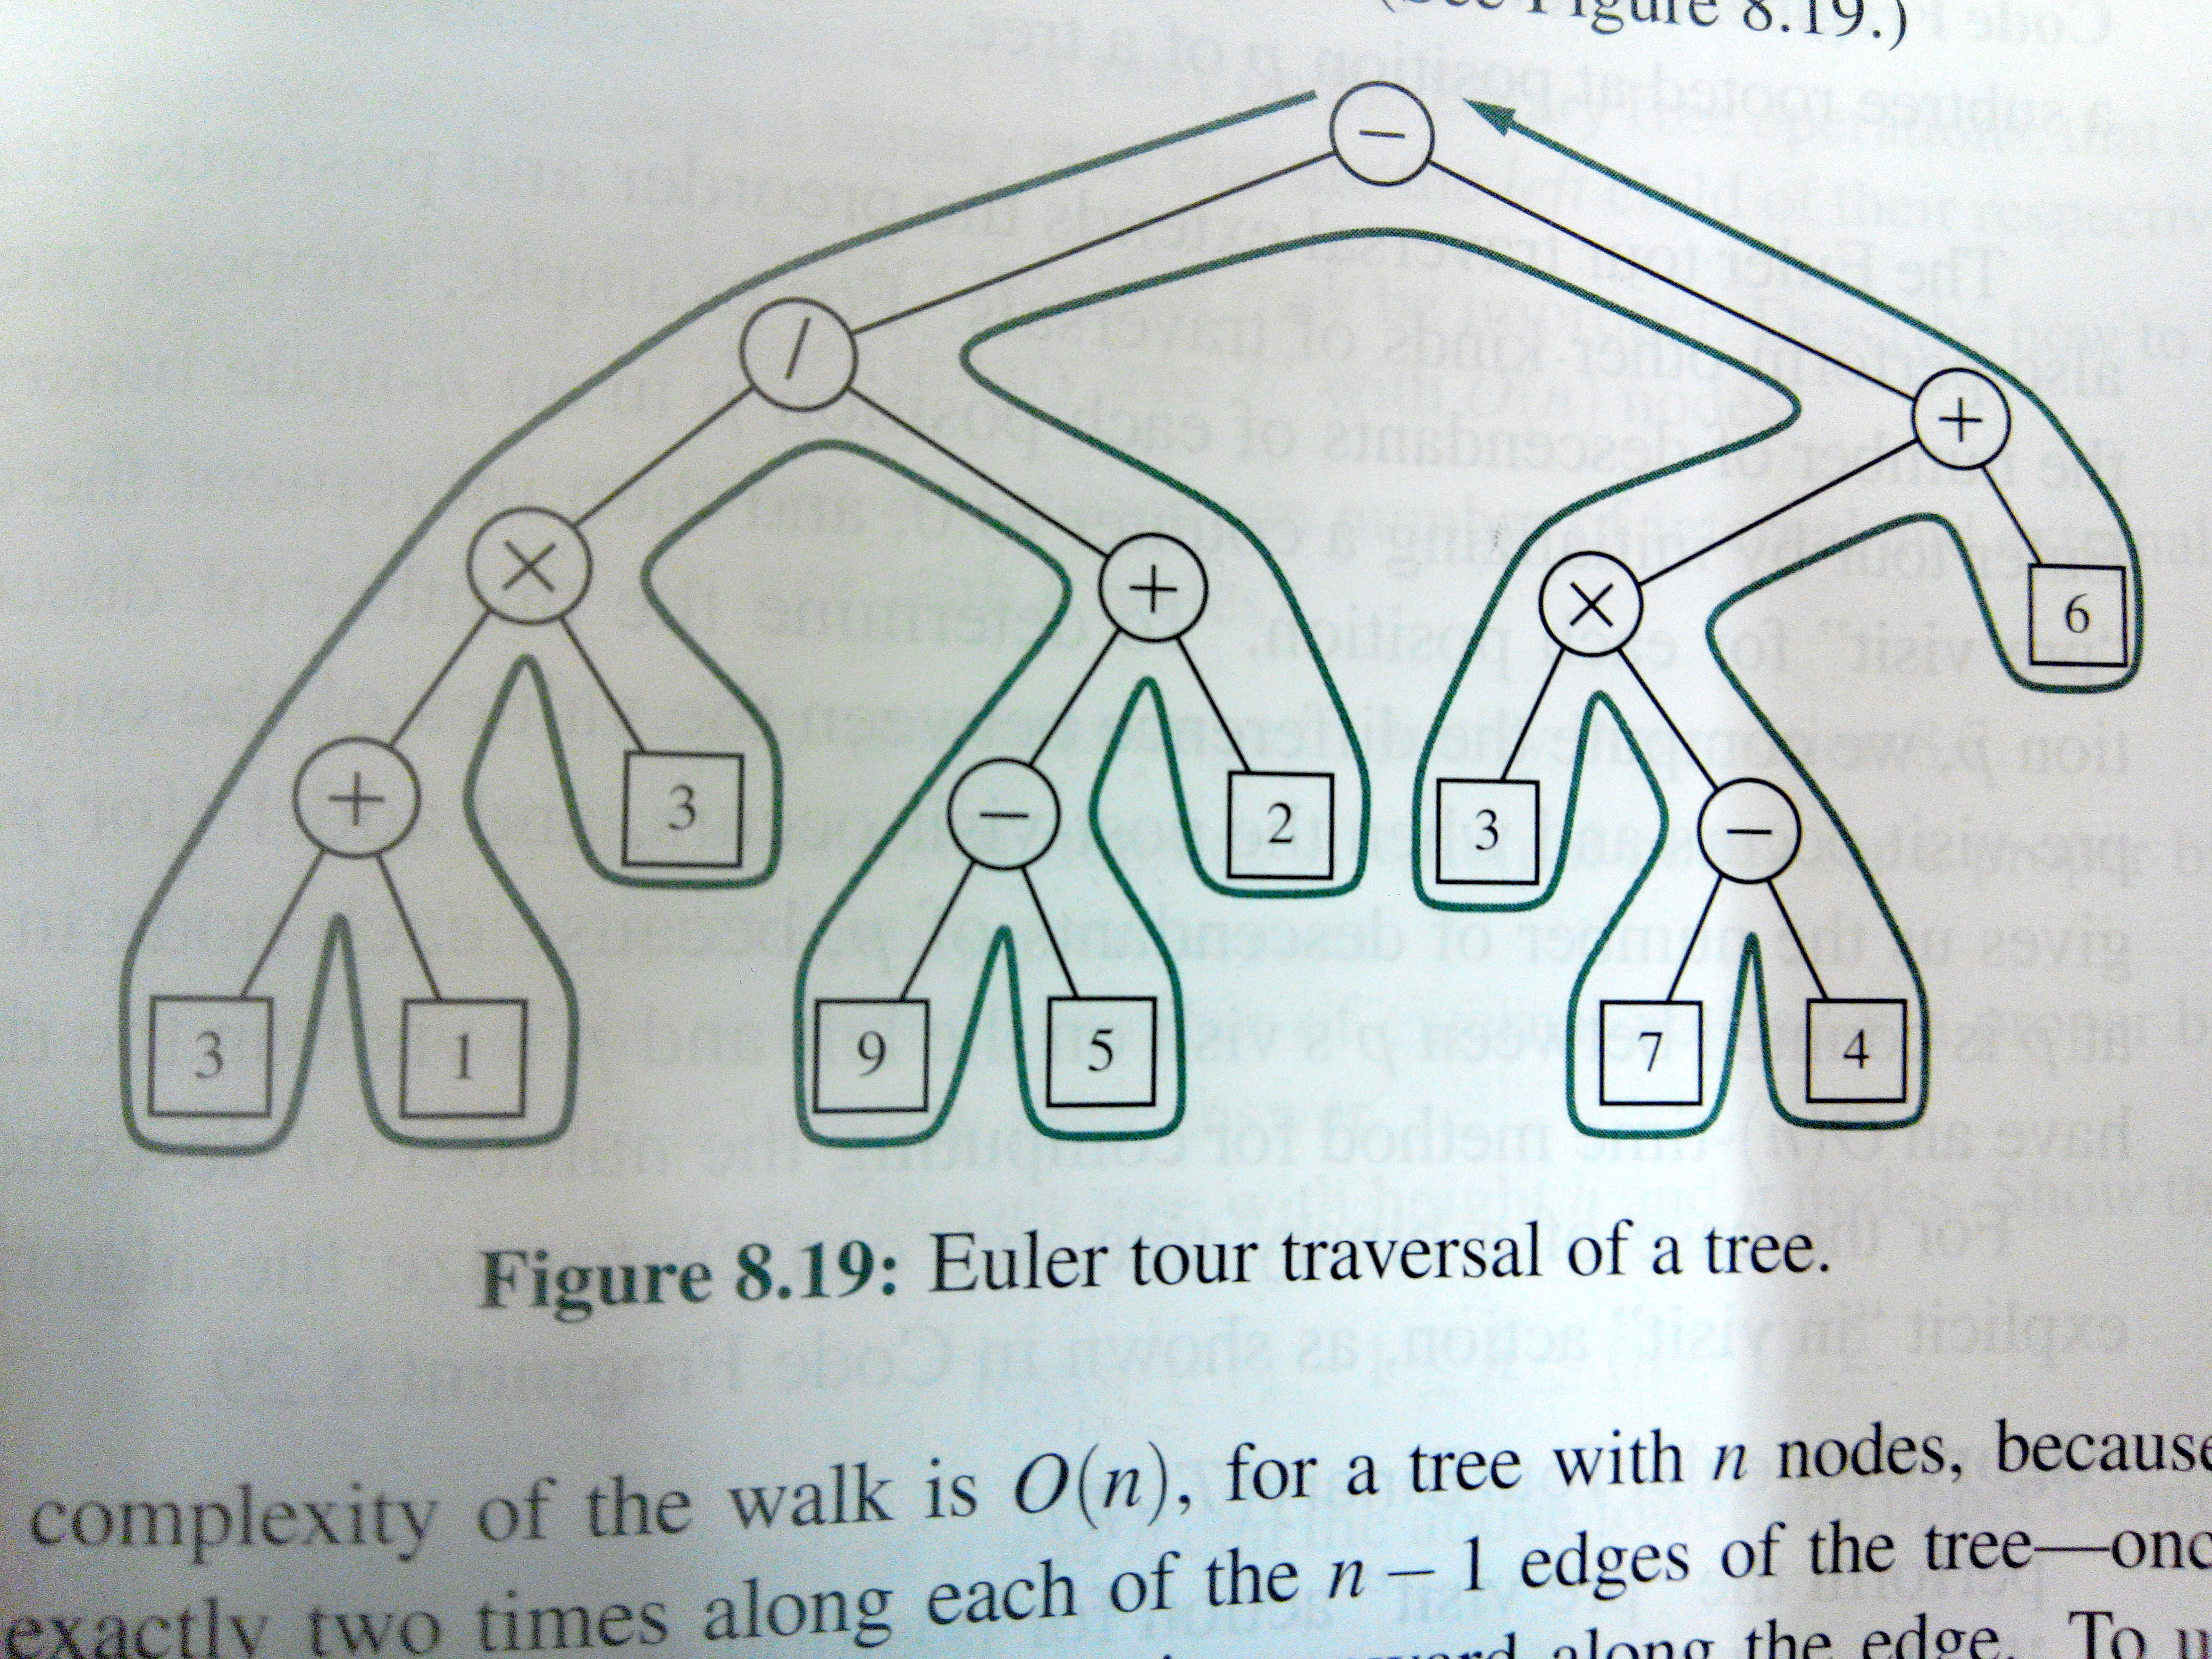
\includegraphics[scale=0.1]{euler.jpg}
\end{figure}
\end{center}

\subsubsection{breadth-first Tree}
Contrairement aux algorithme de traversée en profondeur, celui-ci utilise une liste FIFO, soit une file. \\
\begin{enumerate}
\item Prends tous les noeuds d'un niveau dans une liste fifo
\item Un par un, fait la mm chose en listant les noeuds du niveau suivant
\item et ainsi de suite
\end{enumerate}
Pour mieux comprendre, on peut utiliser le pseudo code suivant:
\begin{verbatim}
ParcoursLargeur(Sommet s):
{
  f = CreerFile();
  f.enfiler(s);
  marquer(s);
  TANT-QUE NON f.vide() FAIRE
      s = f.defiler();
      afficher(s);    
      POUR TOUT voisin de s FAIRE
           SI voisin non marqué FAIRE
                f.enfiler(voisin);
                marquer(voisin);
           FIN SI
      FIN POUR TOUT 
  FIN TANT QUE       
 }
\end{verbatim}

\section{Heaps}
Un heaps est un binary tree qui stocke des entrées directement à leur bonne positions et qui possède 2 propriétées:
\begin{itemize}
\item Dans un heap T, pour chaque positions p autre que la racine, la clé stockée en p est plus grande que la clé des parents de p.
\item Un heap avec une hauteur h est un arbre binaire complet si tous les niveaux  1 -> (h-1) ont le maximum de noeuds possible. Et les noeuds du niveau h, sont au maximum à gauche
\end{itemize}

\section{Priority queue}
Permet de sotcker des objets qui doivent être utilisé dans un ordre bien précis. C'est à dire qu'elle va donner un avantage à certains objets par rapport à d'autres en fonction d'un critère.\\
On ajoute l'élément avec une clé.\\

\begin{itemize}
\item inser(k, v)
\item min()
\item removeMin()
\item size()
\item isEmpty()
\end{itemize}

\subsection{Implémentation}
On peut l'implémenter avec une liste non triée .. plus facile pour ajouter des éléments mais trouver le min, et le remove min sont plus lourd soit en O(n).\\

Pour une implémentation avec une liste triée, on est en O(n) pour ajouter des éléments mais on est en O(1) pour le reste.\\

On peut également l'implémenter avec un heap. Ceci permet d'avoir une complexité d'ajout et de suppression en O(log n )

\section{Map}
Map est un type de donnée abstraite qui permet de stocker efficacement des valeurs grâce à une clé. On stocke donc une paire de données, (k,v) avec la clé k et l'objet v.

\begin{itemize}
\item size()
\item isEmpty()
\item get(k) : retourne l'objet stocké avec la clé k
\item put(k,v) : rajoute une entrée avec la clé K si elle n'existe pas, sinon, la remplace! (attention ça peut faire des dégâts)
\item remove(k)
\item keySet() retourne une collection 'itérable' des clés stockées
\item values() retourne une collection 'itérable' des entrées stockées 
\item entrySet() retourne une collection 'itérable' des clés-entrées stockées
\end{itemize}

\subsection{Sorted Map}
\begin{itemize}
\item firstEntry()
\item lastEntry()
\item ceilingEntry(k) renvoie la valeur la plus proche de k, et plus grand ou égal à k.
\item floorEntry(k)renvoie la valeur la plus proche de k, et plus petite ou égal à k.
\item lowerEntry(k) retourne la valeur juste en dessous de k (<)
\item higherEntry(k) retourne la valeur juste au dessus de k (>)
\item subMap(k1, k2)
\end{itemize}


\section{Hashing}
les but est d'utiliser une fonction de hash pour créer la clé de l'élément dans un tableau.\\
On considère le tableau utilisé comme un bucket array, c'est à dire que si on ne gère pas les collisions, on peut avoir plusieurs éléments dans une 'case'. Pour mettre un éléments, on a plusieurs étapes
\begin{itemize}
\item fonction de hash --> int
\item compression --> 0 <= int < N avec N la taille du tableau
\item gestion des collisions
\end{itemize}

Dans une table de hashing, on défini le facteur de charge (load factor) $\lambda = n/N$ avec n le nombre d'éléments dans la bucket array tandis que N sa taille.


\subsection{Collisions}
\subsubsection{Sparate chaining}
Le but est d'utilise comme une seconde collections dans chaque éléments de la bucket array. Par exemple, un autre tableau, ou une liste chainée.

\subsubsection{Linear probing}
Si la place est déjà prise on regarde la suivante jusqu'à ce qu'on en trouve une de libre.

\subsubsection{Quadratic probing}
Si la place A[h(k)] est prise, on regarde en A[h(k) + $i^2$] avec i = 1, 2 ...\\
Attention, ça cause des problèmes dès que le tableau est rempli à moitié, on est pas sur de trouver des places :(

\subsubsection{Double hashing}
A pour interet de ne pas causer de clusturing mais est bien plus compliqué et implique la dérivée de la table de hash


\subsubsection{Attention suppression d'un élément}
Attention, lors de la suppression d'un élément qui utilise par exemple le linéar probing, on doit transférer tous les éléments suivant dans une autre collection jusqu'à avoir une élément vide. Ensuite il faut les ajouter un à un dans la collection de départ.


\section{Dictionnaire}
Le dictionnaire est une Map avec des strings comme identifiant. (pas sur)

\section{Skip List}
La skip list est une amélioration de liste chainée triée. \\
En fait c'est un ensemble de niveau de liste. chaque élement à une certaine probabilité de se trouver au niveau supérieur.

\begin{figure}[!h]
\begin{center}
\includegraphics[scale=0.4]{skip-list.png}
\caption{Exemple d'une skip list}
\end{center}
\end{figure}

Pour ce qui est de l'algorithme de recherche, au début, on commence en "haut à gauche", et lorsqu'on atteind le dernier éléments, on descend de niveau par rapport à l'élément juste en dessous de celui recherché.
On continue jusqu'à le trouver et si ce n'est pas le cas, on renvoie null.\\
Pour l'ajout d'un élément, on ajoute au bon endroit, on "randomize" pour trouver la taille de la tour et ensuite on la lie aux différents éléments.\\
Pour l'ajout d'élément, c'est la même chose ... il faut faire attention à bien refaire les liens.

Une Skip List est une implémentation possible pour un dictionnaire non ordonné mais il n'est pas judicieux de l'utiliser. Car le système de rangement des entrées est basé sur de l'aléatoire. Donc la recherche se fait en O(log n), l'insertion en O(log n) et la suppresion en O(log n).

\section{Binary seach trees}
\begin{itemize}
\item get(k)
\item put(k, v)
\item remove(k)
\end{itemize}

\section{Balance Search Trees}
Le but est d'utiliser des algo pour l'ajout et la supression de manière à garder un arbre le plus équilibré possible.

\subsection{Rotation}
La rotation à pour but de changer de place entre la formation de gauche et la formation de droite :
\begin{figure}[!h]
\begin{center}
\includegraphics[scale=0.4]{rotation.jpg}
\caption{exemple de rotaion}
\end{center}
\end{figure}

Bien sur ces changements ce font lorsqu'ils sont nécéssaire pour rebalancer un abre. Pour ça en fait on définit 3 fonctions, qu'on verra plus spécifiquement dans les différente type d'arbres balancé
\begin{itemize}
\item rebalanceInsert
\item rebalanceDelete
\item rebalanceAccess
\end{itemize}

\subsection{AVL trees}
On ajoute au binary search tree, l'obligation d'avoir une hauteur en log(n).
\subsubsection{Insertion}
\begin{figure}[!h]
\begin{center}
\includegraphics[scale=0.4]{insertionavl1.jpg}
\caption{insertion avl ex 1}
\end{center}
\end{figure}
\begin{figure}[!h]
\begin{center}
\includegraphics[scale=0.4]{insertionavl2.jpg}
\caption{insertion avl ex 2}
\end{center}
\end{figure}

Lorsqu'on insert un élement, l'arbre risque de ne plus etre balancé. On utilise une stratégie de recherche et réparation.
\subsubsection{Suppression}
C'est semblable pour la suppression.
\begin{figure}[!h]
\begin{center}
\includegraphics[scale=0.4]{suppressionavl.jpg}
\caption{suppression d'un élément avl}
\end{center}
\end{figure}

\subsection{Multiway search tree}
Prenons W, un noeud d'un arbre ordonné. On dit de w qu'il est un d-node s'il possède d enfants. 
\begin{itemize}
\item Chaque noeud interne de T, doit au minimum posséder 2 enfants.

\item Si on a un noeud w de T qui possède d enfants, tq $c_i$ est un enfant du noeud avec i= 1, ...  ,d . Alors w doit posséder un set de (n-1) paire de clé-valeur (k,v).

\item On défini deux éléments, $k_0$=-$\inf$ $k_d$=$\inf$ (je n'ai pas la moindre idée de leur utilitée :'( ). 
\item Pour comprendre le classement dans ce type d'arbre, il faut prendre un noeud w. Ce noeud possède 'd' enfants appelés $c_i$ avec i = 1, ..., d . On définit par $k_i$ les clés contenues dans le noeud w et k toutes clé contenue dans $c_i$. Le classement est tel que $k_{i-1} \leqslant k \leqslant k_i$.
\end{itemize}

On peut implémenter cet arbre comme une liste simplement chainée et chaque noeud comment une SortedTableMap.

\subsection{(2,4)-tree}
\begin{itemize}
\item chaque noeud interne à au maximum 4 enfants
\item Tous les noeuds externes on la même hauteur
\end{itemize}

Les noeuds ont donc 2, 3 ou 4 enfants et à pour interêt d'utiliser moins d'espace mémoire.

\subsection{B-tree}
Un B-tree d'ordre d est un arbre (a,b) tq a = d/2 et b = d.\\
Soit un arbre ($\frac{d}{2}$, d).

\subsection{Splay tree}
On ajoute aucune règle spécifique à la taille/hauteur de l'arbre mais on va juste modifier la façon d'ajouter, de supprimer ou de rechercher des éléments de manière à garder les éléments les plus recherché au plus près possible du root (splaying) et donc obtenir un algo de recherche plus efficace.

On peut par exemple faire une promotion avec un zig-zig, zig-zag, zig:
\begin{figure}[!h]
\begin{center}
\includegraphics[scale=0.4]{zig-zig.jpg}
\caption{Promotion de x avec un zig-zig}
\end{center}
\end{figure}
\begin{figure}[!h]
\begin{center}
\includegraphics[scale=0.4]{zig-zag.jpg}
\caption{Promotion de x avec un zig-zag}
\end{center}
\end{figure}
\begin{figure}[!h]
\begin{center}
\includegraphics[scale=0.4]{zig.jpg}
\caption{Promotion de x avec un zig}
\end{center}
\end{figure}

\textbf{When to splay ???}
Si on fait une recherche de k, qu'on le trouve alors on le splay pour qu'il devienne le root (pas sur). Sinon, on splay le parent de la feuille (si on le trouve pas .. on arrive à une leaf).\\
Lors d'une insertion, de sorte que le numéro inséré devienne le root --> on l'ajoute et puis on splay.\\
Quand on supprime un élément, on splay le parent de sorte à ce qu'il devienne le root

\section{Pattern Matching algorithms on pattern}

\subsection{Brute force}
On test juste pour chaque lettre, cet algo est loin d'être efficace

\subsection{The Boyer-Moore Algo}
\url{https://www.youtube.com/watch?v=PHXAOKQk2dw}
Permet d'éviter une fraction signifiante du text:\\
Si on a une lettre c qui n'apparait pas du tout dans le pattern, alors on skip le pattern juste après.\\
Si on a un caractère c, qui apparait dans le patern, on skip jusqu'a ce caractère et ensuite on continue.
Pour l'implémentation, c'est un peu différent, On doit créer le tableau de boyer-Moore:\\
Pour ce faire, en partant de la gauche, pour chaque caractère on calcul max(1,length-1-index).
Si il y a plusieurs valeurs, on oublié la plus vieille valeur et on la remplace par la nouvelle.\\
Lors de la comparaison, on commence par la droite et on vas vers la gauche, lorsqu'il y a un mismatch, on décale de la valeur trouvée vers l'avant.

\subsection{The Knuth-Morris-Pratt Algo}
On se rend compte que dans les algorithmes précédents on perd de l'information et on doit la recalculer à chaque fois.\\
Il faut calculer une fonction d'échec : "failure function"
c'est à dire un tableau dans lequel on compte les lettre du début:

\begin{figure}[!h]
\begin{center}
\includegraphics[scale=0.07]{KMP.jpg}
\end{center}
\end{figure}
Ensuite on test. Quand on a un mismatch, on regarde la valeur, donc on recommence à cette valeur.

\section{Pattern Matching algorithms directly on the text}

\subsection{Tries}
Le premier élément n'est pas un caractère.
\begin{figure}[!h]
\begin{center}
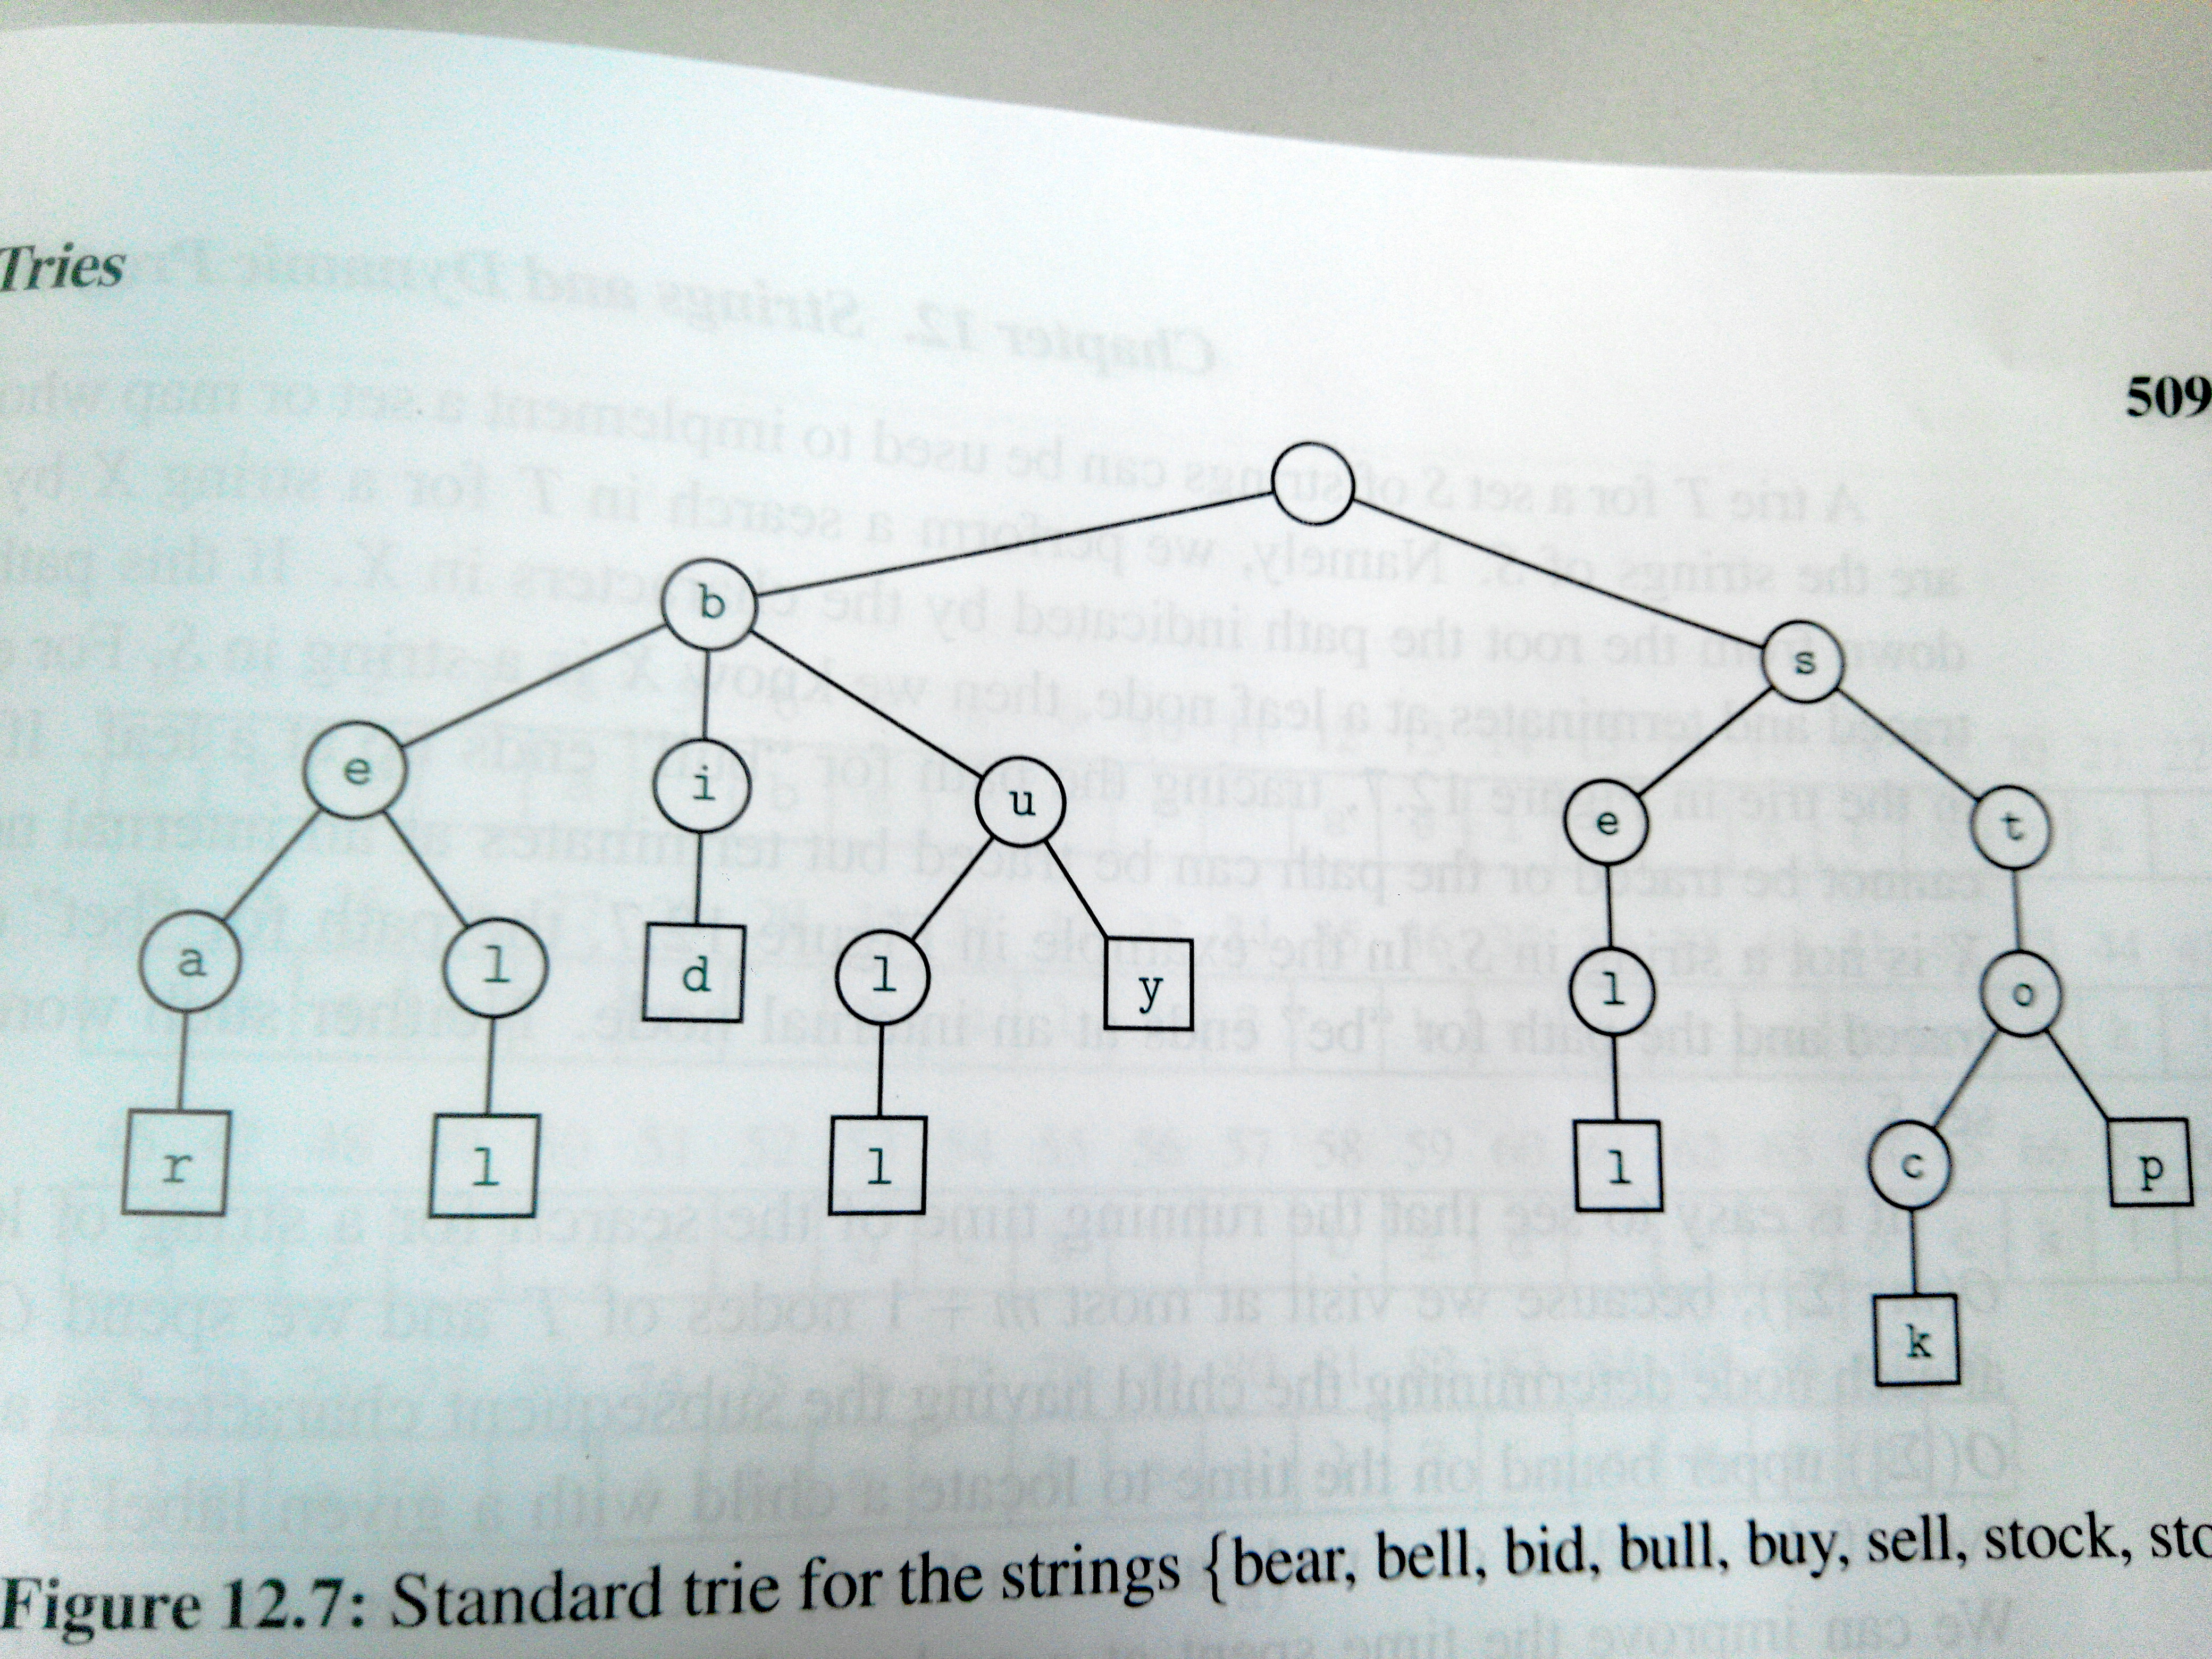
\includegraphics[scale=0.07]{tries.jpg}
\end{center}
\end{figure}
Ensuite, chaque noeud est un caractère de l'alphabet, tq chaque leaf représente un mot. Soit pour retrouver ce mots, il suffit de concaténer tous les strings précédents.


\subsection{Compressed trie}
Le but est que ça prenne moins de place.\\
Parfois c redondant, donc si il n'y a pas plusieur choix de lettre, autant en mettre plusieurs ensemble.\\
Ensuite on peut également stocker une combinaison de 3 index (i,j,k) à la place des string. Ces index sont référencié par rapport à i strings et on en prends les lettres contenues entre l'index j et k.
Cette technique est fort efficace pour réduire l'espace mémoire utilisé.

\subsection{Suffix Tries}
C'est un tries mais uniquement avec les suffix d'un plus grand mot

\section{Greedy method}
C'est une méthode d'optimisation, qui a pour but de faire des choix plus petits et en espérant arriver à une optimisation maximale .. 

\section{Huffman}
\url{https://www.youtube.com/watch?v=ZdooBTdW5bM}\\
Algo utilisé pour compresser du texte.
\begin{enumerate}
\item Premièrement, il faut trouver la fréquence de chaque lettre.
\item On trie le tableau avec comeme clé la fréquence et la lettre en valeur.
\item On utilise une priority queue, on crée un binary tree avec les deux plus petits éléments en les retirant de la priority queue.
\item On rajoute ce tree avec comme clé la somme des deux clés.
\end{enumerate}

\section{graph}
Dans un graphe :
\begin{itemize}
\item vertex (vertices au pluriel)
\item edges
\end{itemize}

\subsection{Comment stocker le graphe}

\begin{itemize}
\item \textbf{Edge list :}
 On crée bêtement une list de noeuds non ordonnée, et une liste non ordonnée d'arrêtes.
\item \textbf{Adjacency list :}
 On crée deux collections, une collection primaire pour stocker les noeuds, et chaque noeud v possède une collection secondaire, I(v) contenant toutes les arrêtes incidentes à ce noeud.
\item \textbf{Adjacency map :}
 Stocker pour chaque noeud, une map (vertex, edge). Avec tous les noeuds adjacent à celui-ci.
\item \textbf{adjacency matrix :}
On crée un tableau à 2 dimensions, on détermine un index par noeud. et on mets dans le tableau l'arrête qui lie les 2 noeuds.
\end{itemize}

\subsection{Graph traversal}
Bon dans le livre, ils parlent de mythologie grec ... je ne pense pas que ça soit important :)

\subsubsection{Depth-First Search (DFS)}
Pour ce faire, on se muni d'une corde, (non on ne vas pas se pendre pour un cours pareil ;) ). On choisi un noeud au hasard. On le colorie pour dire qu'on est passé, ensuite, on prend un des chemins possible (edge) en déroulant la corde, on arrive à une autre noeud, qu'on colorie également. \\
Si l'arrête mène à un noeud déjà visité, on y va pas. Dans le cas, où il n'y a plus d'arrêtes non visitées pour un noeud, alors, on revient sur sont chemin en rebobinant la corde. On arrive au noeud précédent, on regarde s'il y a des noeuds non visités. Ainsi de suite jusqu'a revenir au noeud de départ.\\

\texttt{Cet algo permet de :}  
\begin{enumerate}
\item Voir si un graphe est connexe.
\item Trouver tous les composants connexe d'un graphe.
\item Voir si un graphe possède des cycles ou pas.
\end{enumerate}

\subsubsection{Breadth-First Search (BFS)}
C'est le même algo que le DFS sauf qu'on considère qu'on a plusieurs explorateurs.

\subsection{Transitive Closure}
Le but est de créer un graphe G* en partant de G. Uniquement en ajoutant des arcs (edge) entre le noeud de départ et tout les noeuds qu'il peut joindre de façon indirecte.

\subsection{Directed Acyclic Graphs \& topological ordering}
Premièrement dans beaucoup d'application, il peut être interessant d'avoir un graphe dirigé ne possédant pas de cycle.\\
De plus, on a une topologie ordonnée lorsque que pour chaque edge $(v_i, v_j)$ on a que i<j.

\subsection{Shortest Paths}
Pour ce faire, on travail usuellement avec des "weighted Graphs".
\subsubsection{Dijkstra}
\url{https://www.youtube.com/watch?v=gdmfOwyQlcI}
Cette méthode montre la puissance du "greedy method pattern".\\
On définit V comme étant le set des Vertices du graphe.
\begin{enumerate}
\item On définit s $\in$ V comme étant le noeud de départ.
\item Pour v $\in$ V, on définit D[v] comme étant la distance approximaticve entre s et V. Soit D[s] = 0 et D[u $\in$ V et différent de s]= $\inf$.
\item On définit C comme étant le "Cloud" qui initialement ne contient que s.
\item On choisi u tq u $\in$ V et u $\notin$ C et que D[u] soit le plus petit possible. On ajoute u à C.\\
Attention, u ne doit pas obligatoirement être adjacent au dernier noeud utilisé, mais dois avoir la plus petite valeur de D et ne pas encore avoir été visité.
\item On met à jour D[] car il y a peut-être un meilleur chemin. Ce principe d'amélioration de l'approximation à chaque itération s'appelle la "procédure de relaxation".
\begin{verbatim}
if D[u] + w[u,v] < D[u] then
   D[u] = D[u] + w(u,v)
\end{verbatim}
\end{enumerate}

Pour ce faire, on a le choix entre 2 implémentations, avec une priority queue ou avec un heap.\\
S'il y a peu de noeuds $\rightarrow$ on utilise on heap\\
s'il y a beaucoup de noeuds $\rightarrow$ on utilise une priority queue.\\

Par contre, cette technique cacule la distance mais pas le trajet ... pour pouvoir se souvenir du trajet, on utilise un "shortest-path tree".

\subsection{Minimum spanning tree}
Par exemple, si nous voulons connecter tous les ordinateurs d'un immeuble tout en utilisant le moins de cable possible.\\
Pour définir celà, on dit juste que la somme des poids des différentes arrêtes doit être minimale. c'est le MST problem.

\subsubsection{Prim-Jarnik's algorithm}
\url{https://www.youtube.com/watch?v=bxmnOFxKXY0}\\
Cet algorithme est aussi basé sur la greedy method.
\begin{enumerate}
\item On choisi un noeud.
\item On regarde tous les chemins possible de prendre.
\item On prend celui avec le poids minimum.
\item On regarde tous les chemins non utilisé et adjacent à au moins un noeud déjà visité.
\item On prend celui avec le poids minimum.
\item On réitère l'opération jusqu'à ce que tous les noeuds aient été visités.
\end{enumerate}

\subsubsection{Kruskal's algorithm}
\url{https://www.youtube.com/watch?v=71UQH7Pr9kU}\\
Pour ce faire on ne part pas d'un noeud mais on utilise une priority queue sur les vertex.\\
A chaque itération, on prends l'arrête avec le poids minimum. Cette arrête ne peux pas créer de cycle. soit si e crée un lien $\in$ S, le set des noeuds déjà visités, alors on ne le prends pas. On continue d'itérer jusuqu'à ce que chaque noeud soit connecté ensemble (soit avoir un graphe connexe).
\subsubsection*{Disjoint partitions}
Pour implémenter l'algo de kruskal, il est parfois intéressant de savoir manipuler des sets disjoints. Pour ce faire, on crée des sous arbre contenant des subgraphs, un élément doit se trouver dans un et un seul set.\\
On crée deux grandes fonctions importantes :
\begin{itemize}
\item \textbf{find(x) :} Qui donne le set qui contient x.
\item \textbf{union(T1,T2) :} Qui fait l'union de deux sets disjoints.
\end{itemize}

\end{document}